\chapter{Theoretical background}
In this chapter we focus on how we can generate an arbitrary potential for a cloud of ultracold atoms. To understand it, we first need to review the basics of quantum optics that explain how atoms and light interact. We will see that this interaction creates a dipole force that can be used to trap the atoms. We will then focus on the theory of spatial light modulation. For it, we will present a discussion on Fourier optics and use it to understand how a phase plate can be used for such a purpose.

\section{Atom-light interaction}
At the quantum level, the interaction is usually interpreted as the absorption or emission of photons by the atoms. Despite this picture being accurate, matter can also interact with light through virtual absorption or emission processes, which have interesting behaviours. For this to happen, the frequency of light must be far detuned from the excitation energy of the atoms. An important effect of this type of interaction is the dipole force exerted by light on atoms. To understand the origin of this force, it is sufficient to remember that photons, besides energy, also carry momentum. When a photon is scattered by an atom, its momentum is transferred, generating an effective force that acts on the latter.

\subsection{The dipole force}

To study this force in more detail, we present a discussion adapted from Jonathan Home's lecture notes on quantum optics. Following the standard approach in quantum optics, we model the atom as a two level system, where the energy levels are separated by an energy $\hbar \omega_{eg}$. We also consider light made of a single mode of frequency $\omega / 2\pi$, like the light emitted by a laser. We start by writing the interaction Hamiltonian in the dipole approximation
\begin{equation}
    \label{eq:intH}
    H_\text{int} = - \vec{d} \cdot \vec{E}(\vec{r})
\end{equation}
where $\vec{d}$ is the dipole moment operator, $\vec{E}$ the electric field and $\vec{r}$ the position of the atom. The Hamiltonian of the atom without the interaction term is
\begin{equation}
    H_0 = \frac{\hbar \omega_{eg}}{2} \sigma_z + \frac{\vec
        {p}^2}{2m}
\end{equation}
where $\sigma_z$ is the third Pauli matrix, $\vec{p}$ is the momentum operator and $m$ the mass of the atom.
Furthermore, we consider a classical electric field
\begin{equation}
    \label{eq:Efield}
    \vec{E} = \oh E_0 f(\vec{r} ) \left(e^{i( \vec{k}\cdot\vec{r} - \omega t)} + e^{-i( \vec{k}\cdot\vec{r} - \omega t)}  \right) \vec{\epsilon}
\end{equation}
where $E_0,$ $\omega$ and $\vec{\epsilon}$ are respectively the field strength, frequency and polarization. The function $f(\vec{r})$ allows the field amplitude to vary spatially. Inserting \cref{eq:Efield} in \cref{eq:intH}, the interaction Hamiltonian can be rewritten as
\begin{equation}
    H_\text{int} = (\vec{\mu}_{eg} \cdot \hat{\vec{\epsilon}} E_0) \frac{f(\vec{r})}{2} (\sigma_+ + \sigma_{-}) \left(e^{i( \vec{k}\cdot\vec{r} - \omega t)} + e^{-i( \vec{k}\cdot\vec{r} - \omega t)}  \right)
\end{equation}
where $\mu_{eg} = \bra{e} \vec{d} \ket{g}$. It is now useful to move to the rotating frame with respect to the laser frequency. After transforming the Hamiltonian and performing the rotating wave approximation, we are left with
\begin{equation}
    H = -\frac{\hbar \delta}{2} \omega_z + \frac{\vec{p}^2}{2m} + \frac{\hbar \Omega(\vec
        r)}{2} \left( \sigma_+ e^{i\vec{k}\cdot \vec{r}} +  \sigma_{-} e^{-i\vec{k}\cdot \vec{r} } \right)
\end{equation}
with $\Omega(\vec{r}) = \vec{\mu}_{eg} \cdot \hat{\vec{\epsilon}} E_0 f(\vec{r}) / \hbar$ and $\delta = \omega - \omega_{eg}$.
We can find the resulting force applied on the atom by using Heisenberg's equation of motion
\begin{multline}
    \vec{F} = \frac{\differential\vec{p}}{\differential t} = \frac{i}{\hbar} \left[ H, \vec{p} \right] \\= - \frac{\hbar}{2} \nabla \Omega(\vec{r}) \left( \sigma_+ e^{i\vec{k}\cdot \vec{r}} +  \sigma_{-} e^{-i\vec{k}\cdot \vec{r} } \right) - \frac{\hbar
    }{2} \Omega(\vec{r}) i \vec{k} \left( \sigma_+ e^{i\vec{k}\cdot \vec{r}} -  \sigma_{-} e^{-i\vec{k}\cdot \vec{r} } \right)
\end{multline}
We observe that we get two terms. The first, proportional to the spatial derivative of the field strength, includes a contribution in phase with the light field. It is the term that results in the dipole force exerted by the field on the atom, the one we are interested in. The second term is proportional to the field strength, and it is out of phase of a factor of $\pi$ with respect to the field. It is responsible for the scattering force, essential for cooling atoms. The second term is dominated  by the first for large detuning $\delta$, and it will then be neglected in the following discussion.

We will now make use of two approximation to simplify the calculations. We first make use of a mean-value approximation for the centre-of-mass degree of freedom. This means that we evaluate the internal states operators appearing in $\differential \vec{p} / \differential t$ using the mean position $\vec{r} = \langle \vec{r} \rangle + \langle \vec{v} \rangle t$, where $\vec{v}$ is the velocity of the atom. Moreover, since the timescale on which the internal degrees of freedom of the atom evolve are much faster than the timescale associated to the movement of it, we only consider the steady state solution of the atomic dynamics.
Making use of the approximations explained above, in the limit $\delta  \gg \Omega, \Gamma$, where $\Gamma$ is the decay rate, we find
\begin{equation}
    \vec{F}_\text{dip} = \left\langle \frac{\differential \vec{p}}{\differential t} \right\rangle = - \frac{\hbar}{2} \frac{\Omega}{\delta} \nabla \Omega
\end{equation}
or, in terms of the potential energy,
\begin{equation}
    U = \frac{\hbar}{4}\frac{\Omega^2}{\delta}
\end{equation}
We notice that the dipole force is proportional to the field strength and its gradient, and inversely proportional to the detuning. Moreover, its sign depends on the sign of the detuning. Red-detuned light ($\delta < 0$) generates an attractive potential and can be used to create optical tweezers. This is exploited in our experiment for the creation of the cigar-shaped cloud. On the other hand, blue-detuned light ($\delta > 0$) generates a repulsive potential. This is what we need for the creation of the 2D channel. In the experiment, we use a \SI{660}{nm} laser, blue-detuned with respect to the Lithium atomic transition of \SI{671}{nm}.

\section{Spatial light modulation}
Now that we know how light interacts with atoms, we are interested in the techniques that can be used to arbitrary shape a light beam. At the basis of these techniques there is Forier optics, which will be explained in the next section. We will then look at the different tools that can be used to achieve this goal, focusing on the use of phase plates.

\subsection{Fourier optics}
Fourier optics is essential to understanding how spatial light modulation works. The basic idea  is that a lens returns the Fourier transform of an incident beam on its focal plane. This can be used to transform a phase modulation in an intensity modulation. We will look at this concept in more detail, providing a short introduction to Fourier optics adapted from Saleh and Teich \cite{saleh1991} and Schmidt's previous work \cite{schmidt2021}.

Let's suppose we have a monochromatic wave of wavelength $\lambda$ propagating in the $z$ direction. In the $z=0$ plane, we can denote its complex amplitude with a function $f(x,y)$. The function $f(x,y)$ can be Fourier transformed and decomposed in plane waves propagating in the $x$ and $y$ directions
\begin{equation}
    \label{eq:fourier}
    f(x,y) = \int \differential \nu_x \differential \nu_y F(\nu_x, \nu_y) e^{-2\pi i(\nu_xx+\nu_yy)}
\end{equation}
where $\nu_x = k_x / 2\pi$, $\nu_y = k_y / 2\pi$ and
\begin{equation}
    F(\nu_x,\nu_y) = \int \differential x \differential y f(x, y) e^{2\pi i(\nu_xx+\nu_yy)}
\end{equation}
Each plane wave travels in a direction $(\theta_x, \theta_y)$, where $\theta_i$ is the angle between the direction of propagation and the $z$ axis on the $z-i$ plane, and has an amplitude $F(\nu_x, \nu_y)$. From \cref{eq:fourier}, we find $\theta_x = \sin^{-1}(k_x / k) = \sin^{-1}(\lambda \nu_x$) and $\theta_y = \sin^{-1}(k_y / k) = \sin^{-1}(\lambda \nu_y$).

\begin{figure}
    \centering
    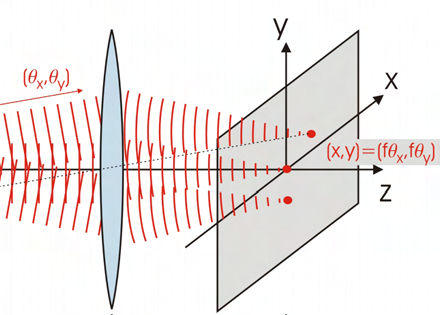
\includegraphics[width=0.6\textwidth]{chapters/chapter_2/figures/fourier.png}
    \caption{Focusing of a plane wave into a point. A direction ($\theta_x, \theta_y$) is mapped into a point $(x,y) = (\theta_x f, \theta_y f)$. The lens in positioned at $z=0$ and the focal plane at $z=f$. Image from Heine \cite{saleh1991}}.
    \label{fig:fourier}
\end{figure}

One way to separate the Fourier components of a wave is by using a lens. A thin spherical lens transforms a plane wave incident on it into a paraboloidal wave focused on a point on the focal plane of the lens (Saleh and Teich Sec. 2.4 \cite{saleh1991}). As shown in \cref{fig:fourier}, a plane wave incident at a small angle $(\theta_x, \theta_y)$ if focused to the point $(x,y) = (\theta_x f, \theta_y f)$, where $f$ is the focal length of the lens. The complex amplitude $g(x,y)$ at $z=f$ is therefore proportional to the Fourier transform of $f(x,y)$ evaluated at $\nu_x = x / \lambda f$ and $\nu_y = y / \lambda f$.
\begin{equation}
    g(x,y) \propto F\left(\frac{x}{\lambda f}, \frac{y}{\lambda f}\right)
\end{equation}
To find the proportionality factor, we trace the propagation of every plane wave in which we have decomposed the input beam through the optical system. Then we integrate over all these plane waves at the output to obtain $g(x,y)$. In the following, we will make use of the Fresnel and paraxial approximations.
A field $F(k_x,k_y)$ can be propagated from the $z=0$ plane to the $z=f$ plane by applying a phase factor $e^{-ik_zz}$
\begin{equation}
    G(k_x, k_y) = F(k_x,k_y) e^{-ik_zz} = H(k_x, k_y, z) F(k_x, k_y)
\end{equation}
with $k_z = \sqrt{k^2 - k_x^2 - k_y^2}$ and  $H(k_x, k_y, z) = e^{-ik_zz}$. We can now perform the Fresnel approximation, which states that for plane waves travelling at small angles ($k_x, k_y \ll k$),
\begin{equation}
    H(k_x, k_y, z) = e^{-ik_zz} = e^{-iz\sqrt{k^2 - k_x^2 - k_y^2}} \approx e^{-ikz}e^{i\frac{k_x^2 + k_y^2}{2k}z}
\end{equation}
$H$ is defined in the Fourier space, so we can bring it back to the real space applying an inverse Fourier transform
\begin{equation}
    h(x,y,z) = \mathcal{F}^{-1}(H(k_x, k_y, z)) = \frac{i}{\lambda z} e^{-ikz} e^{ik\frac{x^2+y^2}{2z}}
\end{equation}
Now we have to take into account the effect of the lens on the beam. A parabolic lens of focal length $f$ will apply a phasor $\phi(x,y) = \exp(-ik\frac{x^2+y^2}{2f})$ in addition to the phase acquired by the propagation of the beam. Overall, at $z=f$, the field is given by the convolution of the two terms
\begin{equation}
    g(x,y) = h(x,y,f) \otimes \left[ \phi(x,y) f(x,y) \right]
    = \frac{i}{\lambda f} e^{-ikf} F\left(\frac{x}{\lambda f}, \frac{y}{\lambda f}\right)
\end{equation}
The proportionality factor (up to a phase factor) is therefore found to be $1/\lambda f$,
and the intensity $I(x,y)$ at the focal plane is
\begin{equation}
    I(x,y) = \frac{1}{(\lambda f)^2} \left| F\left(\frac{x}{\lambda f}, \frac{y}{\lambda f}\right) \right|^2
\end{equation}
To sum up, a lens returns a Fourier transform of the incident beam at a distance equal to the focal length. This can be used to modulate the intensity profile of the beam.

\subsection{Spatial light modulators: the phase plate}
\label{sec:slm_phaseplate}
\begin{figure}
    \begin{subfigure}[t]{0.4\textwidth}
        \centering
        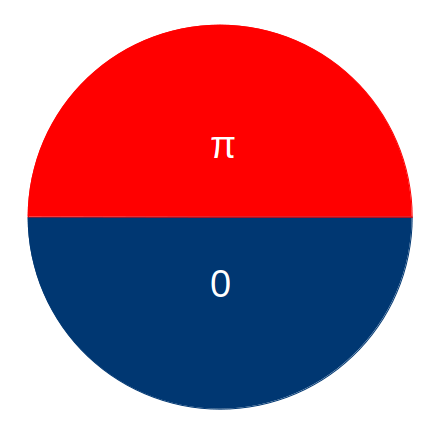
\includegraphics[width=0.8\textwidth, valign=c]{chapters/chapter_2/figures/0pi}
        \caption{$0-\pi$ phase plate}
        \label{fig:0pi_plate}
    \end{subfigure}
    \hfill
    \begin{subfigure}[t]{0.6\textwidth}
        \centering
        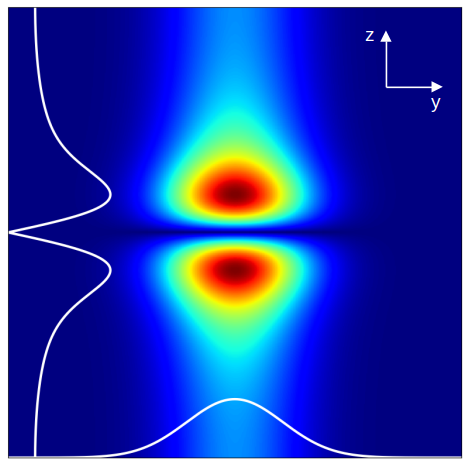
\includegraphics[height=\textwidth, valign=c]{chapters/chapter_2/figures/tem10_sim.png}
        \caption{$\text{TEM}_{01}$ mode}
        \label{fig:tem10}
    \end{subfigure}
    \caption{$\text{TEM}_{01}$ mode generated by o $0-\pi$ phase plate. In the figure on the right, the intensity profile at the focal plane is shown together with the integrated intensity along the two axes.}
    \label{fig:0pi}
\end{figure}
The theory described above can be used as the working principle of numerous devices used for spatial light modulation. Among the ways light can be shaped, it is worth mentioning the use of acusto-optic modulators (AOMs), digital micromirror devices (DMDs), liquid crystals spatial light modulators (LC-SLMs) and phase plates. All these options are good for different purposes. The first three have the advantage of being controllable, allowing the creation of arbitrary shapes simply changing the input signal. The phase plate is cheaper, but once it has been manufactured, it cannot be modified.
The use of an LC-SLM for the creation of a uniform light sheet was investigated by Schmidt in his semester project \cite{schmidt2021}. However, it was found that a phase plate would offer a cheaper and more reliable alternative.

The working principle of a phase plate is very simple. A wave travelling in a transmissive medium has a lower speed than a wave travelling in air. Designing a plate with variable thickness, it is possible to add an arbitrary phase to the beam. The points where the plate is thicker will be delayed with respect to the points where it is thinner. Placing a lens after the plate will result in the desired intensity modulation at the focal plane.
One of the simplest example of phase plates is the $0-\pi$ phase plate, shown in \cref{fig:0pi}. The plate is divided in two halves, with the upper half out of phase by a factor of $\pi$ with respect to the lower half. For a beam propagating in the $x$ direction, the phase profile is then (see \cref{fig:0pi})
\begin{equation}
    \phi(y,z) =
    \begin{cases}
        0 \quad z < 0 \\
        \pi \quad z > 0
    \end{cases}
\end{equation}
This is the phase plate currently used in the experiment, and it generates the $\text{TEM}_{01}$ mode shown in \cref{fig:tem10}.
\begin{figure}
    \begin{subfigure}{\textwidth}
        \centering
        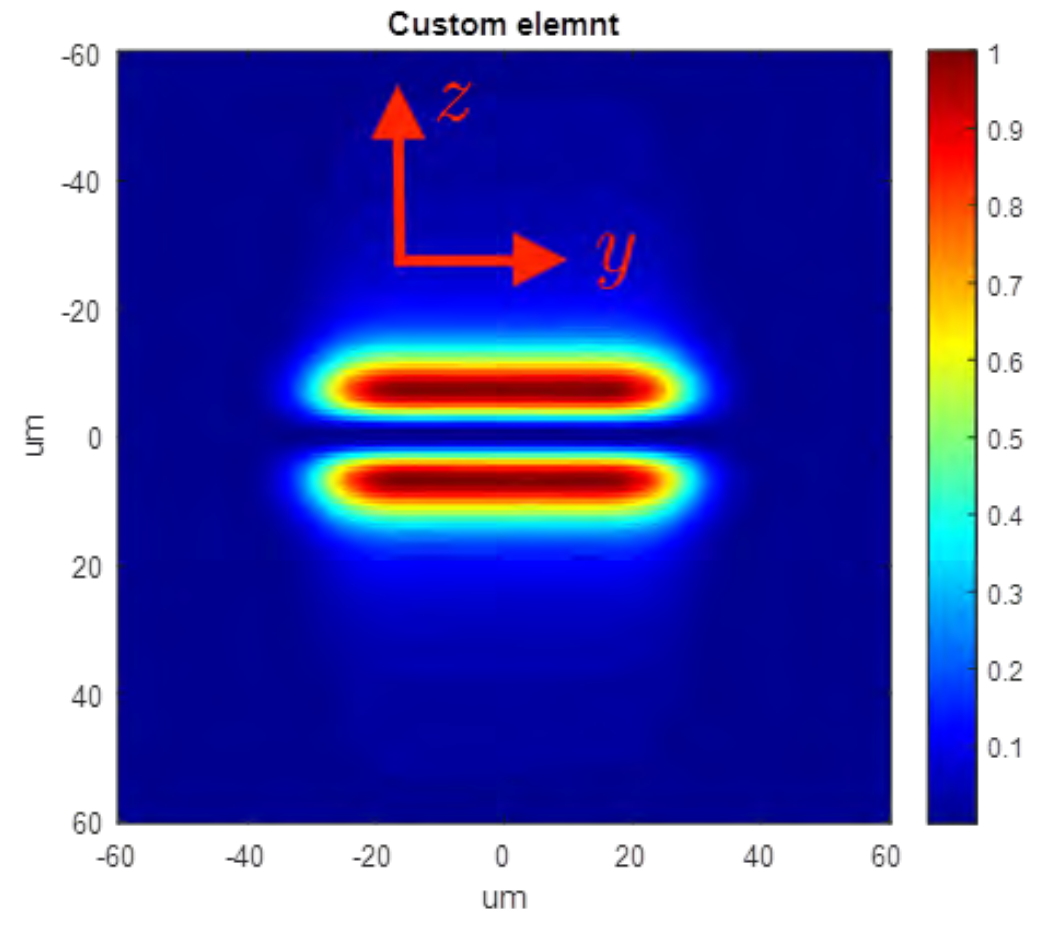
\includegraphics[width=0.7\textwidth]{chapters/chapter_2/figures/tophat.png}
        \caption{Beam profile}
    \end{subfigure}

    \begin{subfigure}{0.5\textwidth}
        \centering
        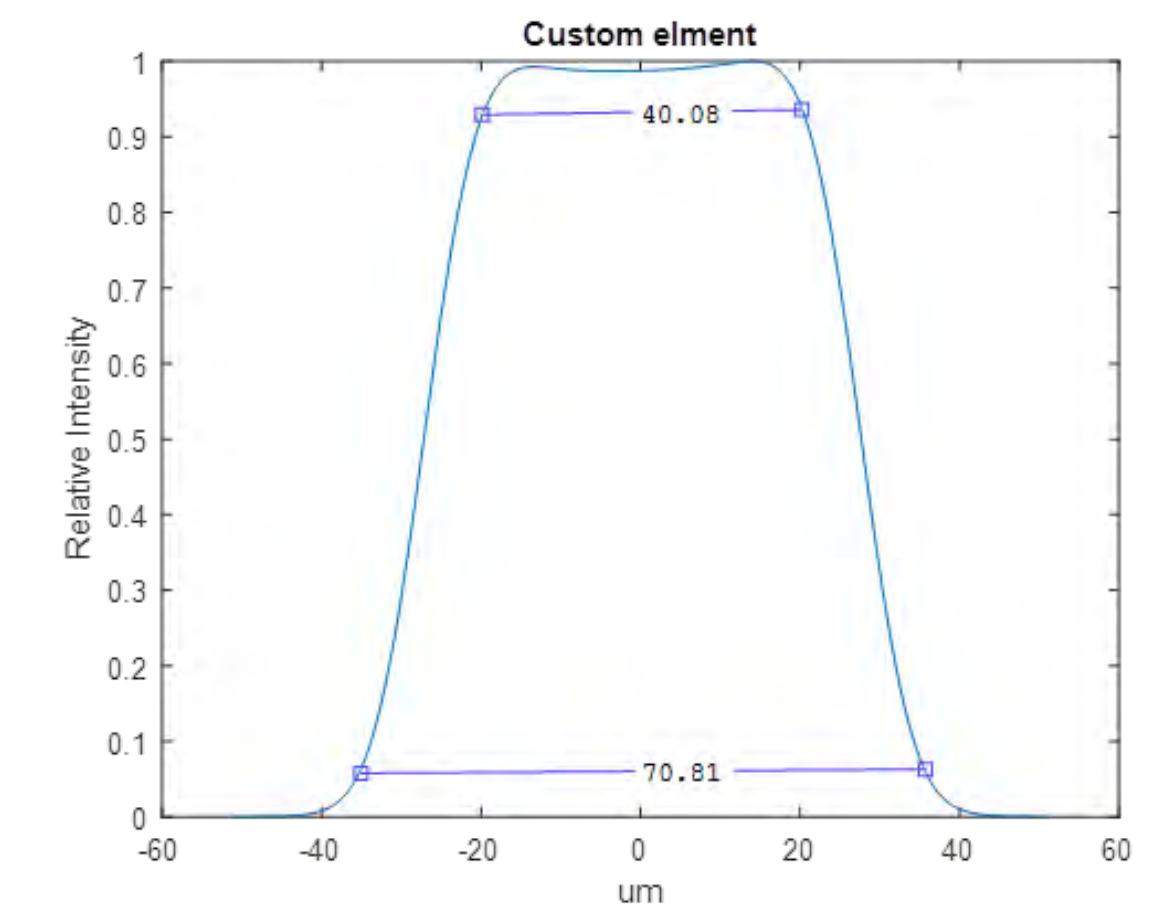
\includegraphics[width=\textwidth]{chapters/chapter_2/figures/tophatx.png}
        \caption{$y$ direction}
        \label{fig:tophaty}
    \end{subfigure}
    \begin{subfigure}{0.5\textwidth}
        \centering
        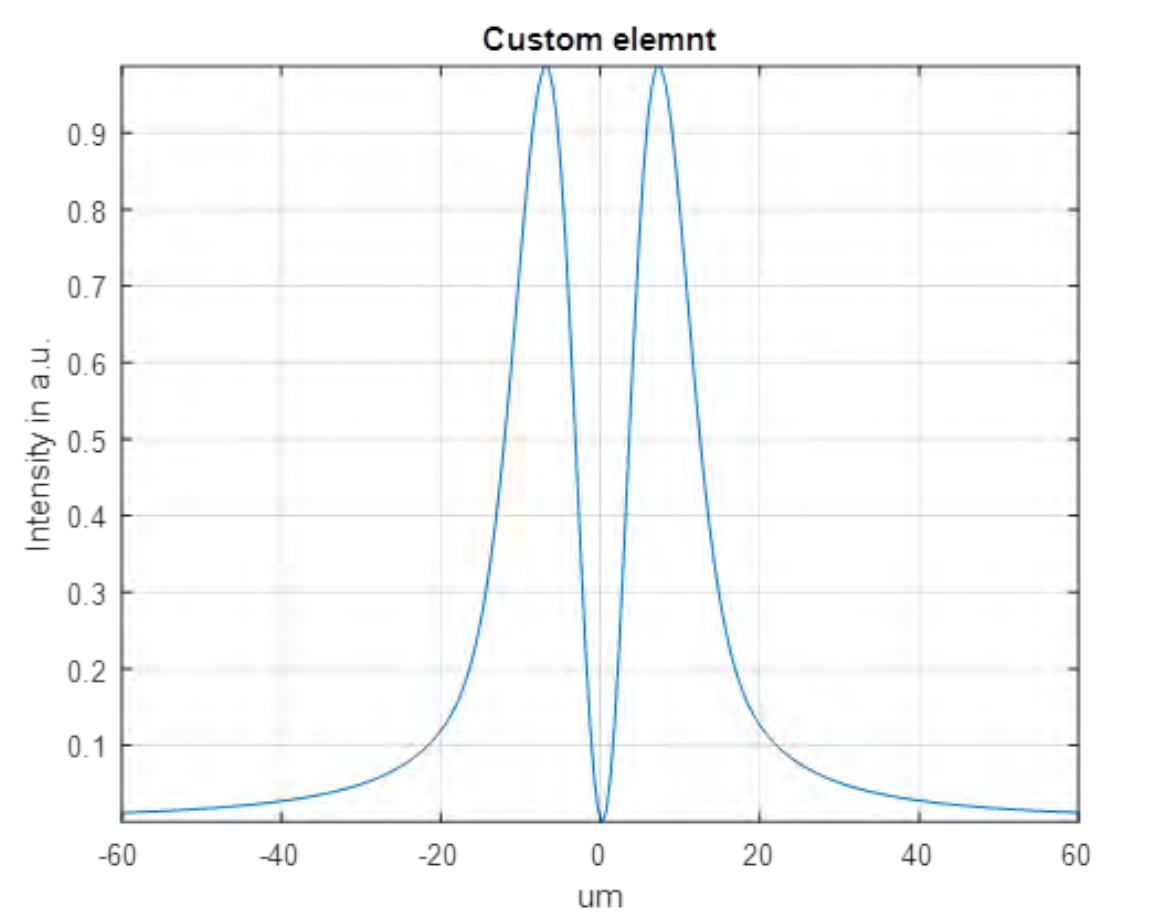
\includegraphics[width=\textwidth]{chapters/chapter_2/figures/tophaty.png}
        \caption{$z$ direction}
        \label{fig:tophatz}
    \end{subfigure}
    \caption{Customized phase plate. In the $y$ direction, the intensity follows a "top hat" profile, characterized by a Gaussian ramping up, a flat region, and a symmetric ramping down. In the $z$ direction, the intensity follows the same profile of a $0-\pi$ phase plate. The image was provided by Holoor, the manufacturing company.}
    \label{fig:tophat}
\end{figure}
As it is clear from \cref{fig:tem10}, the intensity (and therefore the potential) is not uniform along the $y$ direction. On the contrary, it has a Gaussian shape, with a peak at the centre.
What we would like to achieve is a so-called top-hat potential, shown in \cref{fig:tophat}. It differs from the standard $0-\pi$ phase plate in the $y$ direction. Instead of having a Gaussian profile, it initially ramps up from 0 to 1 (in a.u.), then it remains flat in the central region, and it finally decreases back to 0. In the ramp up region, the profile is Gaussian. In the $z$ direction, it generates the same kind of intensity modulation as the $0-\pi$ phase plate. The region we are interested in is the central region. The phase plate was designed to create an intensity profile as uniform as possible, and this is what we have tried to achieve experimentally.

\subsection{Required specifications}
\label{sec:slm_specifications}
We now turn our attention towards the specifications that the phase plate has to satisfy in order to be useful for our experiment. The three main aspects we want to focus on are the width of the flat region, the darkness $D$ and the trapping frequency $\omega_z$.

The phase plate was designed to create a flat region of \SI{40}{\micro \meter}, with a ramp up region of \SI{15}{\micro\meter}. The specifications are relative to the intensity profile generated by the phase plate in combination with a lens of focal length $f=\SI{100}{mm}$. However, in the final experiment it is preferable to use a $f=\SI{250}{mm}$ lens. Therefore all the features will be scaled up by a factor of 2.5. For example the flat region will be \SI{100}{\micro\meter} long instead of \SI{40}{\micro\meter}.

The darkness is the most important parameter of the phase plate. It gives us a measure of how dark is the dark region at the centre of the light sheet compared to the bright region around. Taking inspiration from Krinner's PhD thesis \cite{krinner2015b}, we define it as
\begin{equation}
    \label{eq:darkness}
    D = \frac{I_\text{node}}{(I_\text{max,1} + I_\text{max,2}) / 2}
\end{equation}
where $I_\text{node}$ is the intensity at the nodal plane, and $I_\text{max,1/2}$ is the intensity at the two maxima. For the experiment to work, the darkness has to be on the 0.1\% level. The repulsive laser that creates the 2D channel increases the potential energy with respects to the chemical potential of the reservoirs. If the nodal region is too bright, and therefore the potential energy too high, the atoms will not be able to pass through the channel, and the transport will be suppressed. According to Krinner's work, for a $0-\pi$ phase plate and typical powers of \SI{1.3}{W}, a darkness of one 0.1\% increases the potential energy by \SI{70}{nK}, and the transport is not suppressed.

In order to freeze-out the $z$ dimension, the trapping frequency must be high enough. If we approximate the trapping potential in the neighbourhood of the nodal plane with a second order polynomial
\begin{equation}
    \label{eq:trapping_frequency}
    U(z) = U_0 + \oh m \omega_z^2 z^2 + \mathcal{O}(z^4)
\end{equation}
we require the trapping energy $\hbar \omega_z$ to be higher than the following energy scales \cite{schmidt2021}:
\begin{itemize}
    \item Fermi energy $E_F \approx \SI{600}{nK} = \SI{12.5}{kHz}$
    \item Binding energy, estimated to be smaller than the 20\% of the Fermi energy $E_B \approx \SI{120}{nK} = \SI{2.5}{kHz}$
    \item Temperature $T \approx \SI{60}{nK} = \SI{1.3}{kHz}$
\end{itemize}
Therefore, the phase plate was ordered to have a trapping frequency of at least $\omega_z / 2\pi = \SI{20}{kHz}$, much larger that all the other energy scales.

The final goal of using this phase plate is to have a central region as dark and as uniform as possible. The darkness can be evaluated computing $D$ as explained above in \cref{eq:darkness}. The uniformity of the potential depends on two  things: the intensity variation in the central region and the trapping frequency variation. We can understand it by thinking again at the assumption we made for the potential.
Assuming that the potential is approximately harmonic, we can write it as
\begin{equation}
    U(y,z) = \oh m z^2\omega_z^2(y) + U_0(y)
\end{equation}
where we have explicitly indicated the dependency of $\omega_z$ and $U_0$ on $y$. Assuming the atoms are in the ground state, they will feel an effective potential dependent on $y$
\begin{equation}
    \label{eq:effectivr_potential}
    U(y) = U_0(y) + \oh \hbar \omega_z(y)
\end{equation}
The first term is due to the intensity at the nodal line not being zero. This will add an offset to the potential felt by the atoms. The second term is the energy of the ground state of a harmonic oscillator, where we are assuming again that we can approximate the potential as parabolic in the proximity of the nodal line (see \cref{fig:offset}). What we want to minimize is then the variation of $U(y)$ along $y$, which will depend both on the variation of $U_0(y)$ and of  $\omega_z(y)$.

\begin{figure}
    \centering
    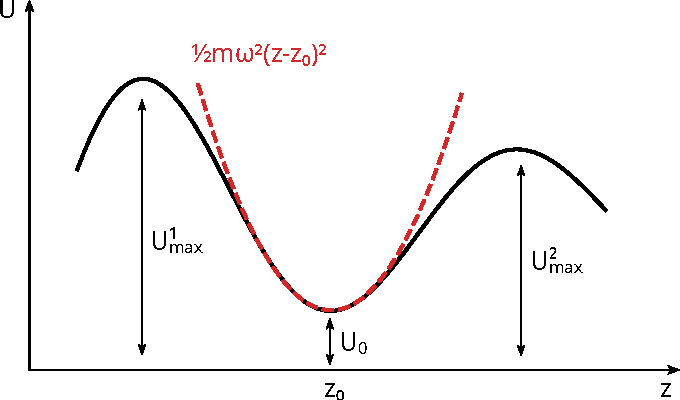
\includegraphics[width=0.7\textwidth]{chapters/chapter_2/figures/offset.pdf}
    \caption{Potential energy along the $z$ direction. At the minimum, a non-zero intensity generates a non-zero potential. In the proximity of the minimum the potential can be approximated as harmonic.}
    \label{fig:offset}
\end{figure}